\documentclass[12pt, a4paper]{article}
\usepackage[utf8]{inputenc}
\usepackage{amsmath}
\usepackage{amsthm}
\usepackage{amssymb}
\usepackage{graphicx}
\usepackage{parskip}
\usepackage{hyperref}
\usepackage{fancyhdr}
\usepackage{lastpage}
\usepackage[vlined,ruled]{algorithm2e}
\usepackage[acronym]{glossaries}
\usepackage{caption}
\usepackage{titlesec}
\usepackage{tikz}
\usetikzlibrary{arrows,automata}

\titleformat{\section}
  {\normalfont\bfseries}{Problem 4.\thesection}
  {0em}{}

\titleformat{\subsection}
  {\normalfont\bfseries}{4.\thesubsection}
  {0em}{}
  
\titleformat{\subsubsection}
  {\normalfont\bfseries}{4.\thesubsection}
  {0em}{}

\title{%
  Stochastic Network Modeling \\
  Homework 4 - Solutions
}
\author{%
  Juan Pablo Royo Sales\\
  \small{Universitat Politècnica de Catalunya}
}
\date\today

\pagestyle{fancy}
\fancyhf{}
\fancyhead[C]{}
\fancyhead[R]{Juan Pablo Royo Sales - UPC MIRI}
\fancyhead[L]{SNM - Homework 4}
\fancyfoot[L,C]{}
\fancyfoot[R]{Page \thepage{} of \pageref{LastPage}}
\setlength{\headheight}{15pt}
\renewcommand{\headrulewidth}{0.4pt}
\renewcommand{\footrulewidth}{0.4pt}

\renewcommand{\qedsymbol}{$\blacksquare$}

\begin{document}

\maketitle

\section{}
\subsection{}
States are:
\begin{itemize}
  \item $H$ When a head shows up
  \item $T$ When a tail shows up
  \item $HH$ When a head shows up after $H$
  \item $TT$ When a tail shows up after $T$
  \item $TTT$ When a tail shows up after $TT$ 
\end{itemize}

\subsection{}
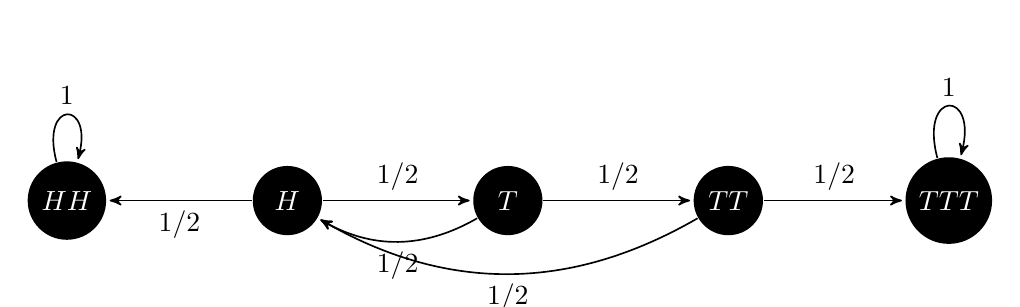
\begin{tikzpicture}[->,>=stealth',shorten >=1pt,auto,node distance=2.8cm,
  semithick]
  \tikzstyle{every state}=[fill=black,draw=none,text=white]

  \node[state]         (A)              {$H$};
  \node[state]         (B) [right of=A] {$T$};
  \node[state]         (C) [left of=A] {$HH$};
  \node[state]         (D) [right of=B] {$TT$};
  \node[state]         (E) [right of=D] {$TTT$};

  \path (A) edge              node {1/2} (B)
        (A) edge              node {1/2} (C)
        (B) edge [bend left]  node {1/2} (A)
        (B) edge              node {1/2} (D)
        (C) edge [loop above] node {1} (C)
        (D) edge [bend left]  node {1/2} (A)
        (D) edge              node {1/2} (E)
        (E) edge [loop above] node {1} (E)
        ;
\end{tikzpicture}

\subsection{}
\begin{align*}
  P = \begin{bmatrix}
       & H & T & HH & TT & TTT\\
   H   & 0 & 1/2 & 1/2 & 0 & 0\\
   T   & 1/2 & 0 & 0 & 1/2 & 0\\
   HH  & 0 & 0 & 1 & 0 & 0\\
   TT  & 1/2 & 0 & 0 & 0 & 1/2\\
   TTT & 0 & 0 & 0 & 0 & 1
  \end{bmatrix}
\end{align*}

\subsection{}
Absorbing states are $TTT$ and $HH$.

\section{}
States are:
\begin{itemize}
  \item $I$: Initial state
  \item $W$: Win $\{7,11\}$ or after second point.
  \item $L$: Loses $\{2,3,12\}$ or after $7$ after point.
  \item $PP$: Player Point.
  \item $CG$: Continue Gambling.
\end{itemize}

\begin{tikzpicture}[->,>=stealth',shorten >=1pt,auto,node distance=2.8cm,
  semithick]
  \tikzstyle{every state}=[fill=black,draw=none,text=white]

  \node[state]         (0)              {$I$};
  \node[state]         (A) [above of=0] {$W$};
  \node[state]         (C) [right of=0] {$PP$};
  \node[state]         (E) [above of=C] {$CG$};
  \node[state]         (B) [right of=C]  {$L$};

  \path (0) edge              node {8/36} (A)
        (A) edge [loop above] node {1} (A)
        (0) edge [bend right=90]  node {4/36} (B)
        (B) edge [loop above] node {1} (B)
        (0) edge              node {24/36} (C)
        (C) edge              node {6/36} (D)
        (C) edge              node {24/36} (E)
        (C) edge              node {6/36} (A)
        (E) edge [loop above] node {24/36} (E)
        (E) edge              node {6/36} (D)
        (E) edge              node {24/36} (A)
        (D) edge [loop above] node {1} (D)
        ;
\end{tikzpicture}
\begin{align*}
  P = \begin{bmatrix}
       & I & W & L & PP & CG\\
   I   & 0 & 8/36 & 4/36 & 24/36 & 0\\
   W   & 0 & 1 & 0 & 0 & 0\\
   L   & 0 & 0 & 1 & 0 & 0\\
   PP  & 0 & 6/36 & 6/36 & 0 & 24/36\\
   CG  & 0 & 6/36 & 6/36 & 0 & 24/36
  \end{bmatrix}
\end{align*}

\begin{subequations}
  \begin{align}
    \pi(0) = (1, 0, 0, 0, 0)
  \end{align}
\end{subequations}

\section{}
\subsection{}

States are:
\begin{itemize}
  \item $F$: Machine Failure
  \item $3MW$: 3 Motors working
  \item $2MW1R$: 2 Motors working 1 Repair
\end{itemize}

Probabilities are:
\begin{itemize}
  \item $P(1R | 2MW1R) = P(1R)P(2W) = \frac{2}{3}\frac{1}{4}$: Probability that 1 continue in repair when 2 is working.
  \item $P(1B | 2MW1R) = P(1B)P(2W) = \frac{1}{3}\frac{1}{4}$: Probability that 1 fail when 2 is working.
  \item The rest are known by the statement.
\end{itemize}

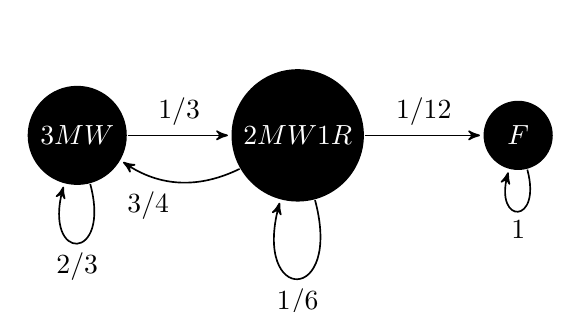
\begin{tikzpicture}[->,>=stealth',shorten >=1pt,auto,node distance=2.8cm,
  semithick]
  \tikzstyle{every state}=[fill=black,draw=none,text=white]

  \node[state]         (3MW)                  {$3MW$};
  \node[state]         (2MW1R) [right of=3MW] {$2MW1R$};
  \node[state]         (F)   [right of=2MW1R] {$F$};

  \path (3MW) edge [loop below] node {2/3} (3MW)
        (3MW) edge              node {1/3} (2MW1R)
        (2MW1R) edge [bend left]  node {3/4} (3MW)
        (2MW1R) edge [loop below] node {1/6} (2MW)
        (2MW1R) edge   node {1/12} (F)
        (F)   edge [loop below] node {1} (F)
        ;
\end{tikzpicture}

\subsection{}
\begin{align*}
  P = \begin{bmatrix}
        & 3MW & 2MW1R & F\\
    3MW & \frac{2}{3} & \frac{1}{3} & 0\\
    2MW1R & \frac{3}{4} & \frac{1}{6} & \frac{1}{12}\\
    F   & 0 & 0 & 1\\
  \end{bmatrix}
\end{align*}

\begin{subequations}
  \begin{align}
    \pi(0) = (1, 0, 0)
  \end{align}
\end{subequations}

\subsection{}
\begin{subequations}
  \begin{align}
    E[T] = T \times \pi(0)P^T
  \end{align}
\end{subequations}


\end{document}

